\documentclass[]{standalone}
%\usepackage{mathptmx}
%\renewcommand{\familydefault}{\rmdefault}
%\usepackage[T1]{fontenc}
%\usepackage[latin9]{inputenc}
\usepackage{siunitx}
\usepackage{array}
\usepackage{amsmath}
\usepackage{ifthen}
\usepackage{pgfplots}
\pgfplotsset{compat=1.14}
\usepackage{titling, graphicx}
\usepackage{tikz}
\usepackage{upgreek}
\usepackage{amsmath,amsthm}
\usepackage{strtikz}
\usetikzlibrary{shapes,arrows.meta,intersections,graphs,graphs.standard}
\usetikzlibrary{math,fit}
\usetikzlibrary{calc,intersections,through,backgrounds,decorations.pathmorphing}


\begin{document}
\begin{tikzpicture}
\pilesupport[%
  x coordinate=0cm,
  y coordinate=0cm,  
  pile depth=5cm,
  pile diameter=1cm,
  pile line thickness=1pt,
  fill color=gray,
  draw boundary line=0,
  boundary line thickness=3pt,
  boundary line color=blue,
  boundary line type=dashed,
  horizontal show springs=1,
  horizontal number of springs = 10,
  horizontal mirror springs=0,
  horizontal space = 0.0cm,
  horizontal start ratio = 0.05,
  horizontal end ratio = 0.05,
  horizontal spring text = {$t-z$ yayları},
  horizontal text color = black,
  horizontal text shiftx=0pt,
  horizontal text shifty=0pt,
  horizontal text location=above,
  horizontal spring prelength ratio=0.2,
  horizontal spring postlength ratio=0.2,
  horizontal spring segment=0.15cm,
  horizontal spring width=3pt,
  horizontal spring scale=1,
  horizontal spring line thickness=1pt,
  horizontal spring color=green,
  horizontal support width=0.3cm,
  horizontal support depth=0.1cm,
  horizontal support line thickness=1pt,
  horizontal show support shade=1,
  horizontal support shade color=red,
  vertical show springs=1,
  vertical number of springs = 5,
  vertical show last spring=0,
  vertical mirror springs=0,
  vertical space = 0.5cm,
  vertical space between springs = 0.1cm,
  vertical start ratio = 0.0,
  vertical end ratio = 0.0,
  vertical spring text = {$p-y$ spring},
  vertical text color = black,
  vertical text shiftx=0pt,
  vertical text shifty=0pt,
  vertical text location=above,
  vertical spring length=0.5cm,
  vertical spring prelength ratio=0.15,
  vertical spring postlength ratio=0.15,
  vertical spring width=0.1cm,
  vertical spring segment=0.15cm,
  vertical spring scale=1,
  vertical spring line thickness=1pt,
  vertical spring color=black,
  vertical support width=0.3cm,
  vertical support depth = 0.1cm,
  vertical support line thickness = 1pt,
  vertical show support shade=1,
  vertical support shade color=blue,
  axial show spring=1,
  axial spring text = {$Q-z$ spring},
  axial text color=black,
  axial text shiftx=2pt,
  axial text shifty=-2.5pt,
axial spring length=1cm,
axial spring prelenratio=0.25,
axial spring postlength ratio=0.1,
axial spring segment=0.15cm,
axial spring width=0.1cm,
axial spring line thickness=1pt,
axial spring color=black,
axial support width=0.3cm,
axial support depth = 0.1cm,
axial support line thickness = 1pt,
axial show support shade=1,
axial support shade color=green,
show frames=0,
frame number=5,
frame circle radius=1pt,
frame line thickness=1pt,
frame line color=blue,
frame line type=dashed,]
%\draw(0,0) -- (4,2);
\end{tikzpicture}
\end{document}